\documentclass[11pt]{amsart}
\usepackage{amsmath}
\usepackage{geometry}                % See geometry.pdf to learn the layout options. There are lots.
\geometry{letterpaper}                   % ... or a4paper or a5paper or ... 
%\geometry{landscape}                % Activate for for rotated page geometry
%\usepackage[parfill]{parskip}    % Activate to begin paragraphs with an empty line rather than an indent
\usepackage{graphicx}
\usepackage{caption}
\usepackage{subcaption}
\usepackage{amssymb}
\usepackage{epstopdf}
\usepackage[]{algorithm2e}
\usepackage{tikz}
\usetikzlibrary{positioning}
\usepackage{intcalc}
\usepackage{blkarray}


\newcommand{\vek}[1]{\mathbf{#1}}

\graphicspath{{Figures/}}

\title{Comp 652: Assignment 3}
\author{Carlos G. Oliver (260425853)}
\date{\today}                                           % Activate to display a given date or no date

\begin{document}
\maketitle

\section{Q1: PCA}

\begin{figure}[h]
\centering
\begin{subfigure}{0.5\textwidth}
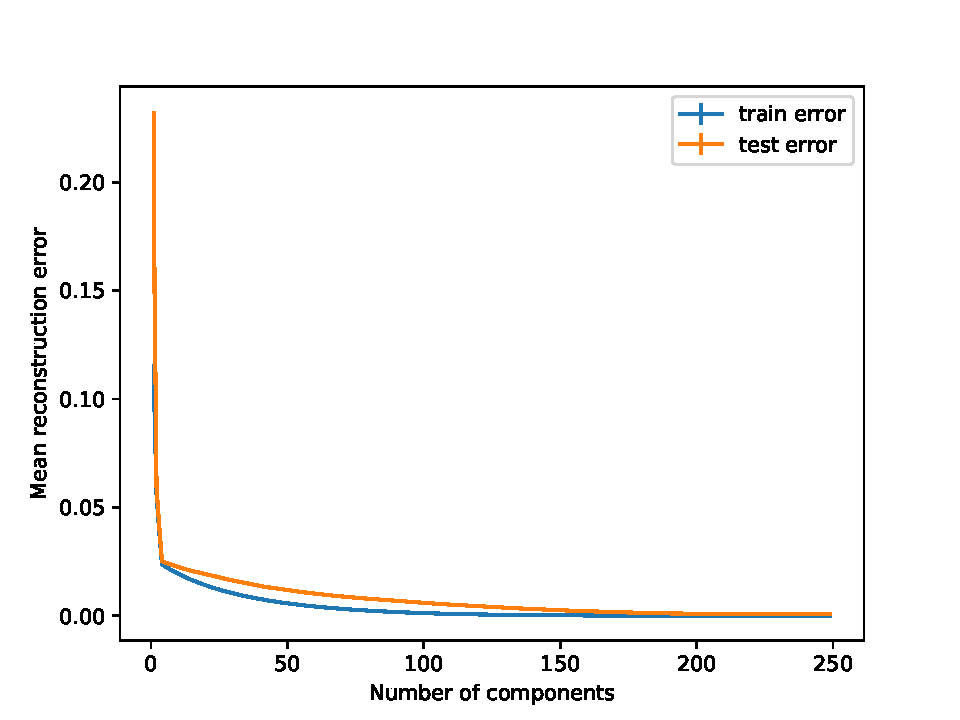
\includegraphics[width=\textwidth]{reconstruction.pdf}
\caption{}
\label{subfig:rfam_count}
\end{subfigure}
~
\begin{subfigure}{0.46\textwidth}
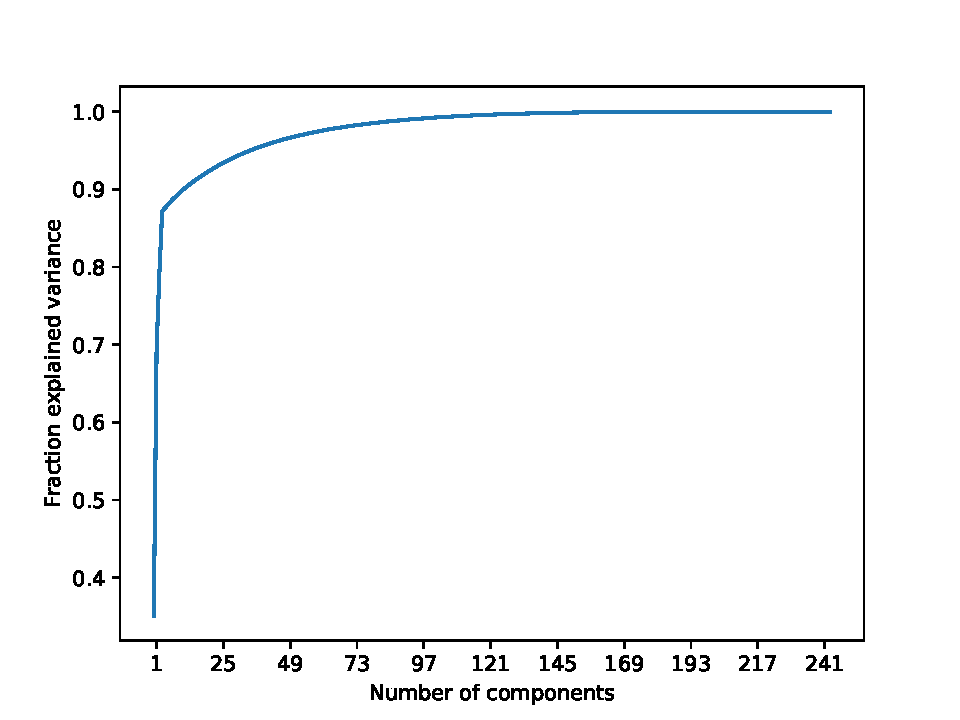
\includegraphics[width=\textwidth]{var.pdf}
\caption{}
\label{subfig:rfam_stats}
\end{subfigure}

\caption{}
\label{fig:rfam}
\end{figure}

\section{Q2: Spectral methods for weighted automata}
\subsection{(a)}

We use a property of Hankel matrices which is: if $\text{rank}(H_f) = n \Rightarrow$ there exists a weighted finite automaton $\mathcal{A}$  with $n$ states such that $g = g_{\mathcal{A}}$ for some function $g : \Sigma^{*} \rightarrow \mathbb{R}$ where $\Sigma^{*}$ is the set of all strings that can be generated from alphabet $\Sigma$. In this example, the function $g$ counts the number of $1$s in a string generated from $\Sigma = \{0, 1\}$ the Hankel matrix $H_g$ would take the form: 


 
\[
H_g = \begin{blockarray}{cccccc}
\def\ra{\color{red}\ba}
 & \lambda & 0 & 1 & 11 & \hdots \\
\begin{block}{c[ccccc]}
  \lambda & 0 & 0 & 1 & 2 & \hdots \\
  0 & 0 & 0 & 1 & 2 &  \\
  1 & 1 & 1 & 2 & 3 &  \\
  11 & 2 & 2 & 3 & 4 &  \\
  111 & 3 & 3 & 4 & 5 &  \\
  110 & 2 & 2 & 3 & 4 &  \\
  \vdots & \vdots &  &  &  & \ddots \\
\end{block}
\end{blockarray}
\label{mat:h_1}
 \]

The above matrix is arranged so all possible strings composed only of $1$s, $Q = \{1\}^N \quad \forall N \in \mathbb{Z^+}$ precede all other strings ($\Sigma^{*} - Q$) with the exception of $\{0\}^1$ and $\lambda$. If we order prefixes and suffixes in S in increasing $N$ we can easily see that any row $m$ in this sub block $H^{1}_g$ of $H_g$ is a linear combination in the form $H^{1}_g(m, \cdot) = 2H^{1}_g(m, \cdot) - H^{1}_g(m-1, \cdot)$. The remaining entries in $H_g$ are formed by prefixes and suffixes containing $0$s which do not contribute to the evaluation of $g$ and therefore can also be obtained from rows or columns in $H^{1}$. Therefore the rank of $H_g$ is 2 where only the $\lambda$ or $\{0\}^1$ and the $\{1\}^1$ contribute to the row rank. The same can be shown for the column rank.

\subsection{(b)}

If $f$ is a probability distribution over $\Sigma^*$ then we have $\sum_{s \in \Sigma^*} f(s) = 1$ gives a probability for every string in $\Sigma^*$. Then $f_{sub}(w)$ is the probability that the string $w$ occurs in any word generated by $\Sigma^*$ since $u$ and $v$ represent all possible prefixes and suffixes to the word $w$.

\subsection{(c)}

Let $ \Sigma_{w \in \Sigma^*} A_w \equiv S$.

\begin{equation}
\begin{aligned}
S = (I - A_0 - A_1)^{-1} = (I - A_0 - A_1) S          &= I \\
				       (I - A_0 - A_1)SS^{-1} &= S^{-1}	\\
				       (I - A_0 - A_1)^{-1} 	&= S
\end{aligned}
\end{equation}

Now we use this identity to compute the sum of the function $f$ over all words as $ \Sigma_{w \in \Sigma^*} f(w)$. We can express the function over a string as

\begin{equation}
\begin{aligned}
f(w) = \alpha_0^T Aw \alpha_{\infty}
\end{aligned}
\end{equation}

So for all the words we have
\begin{equation}
\begin{aligned}
\sum_{w \in \Sigma^*} f(w) &= \sum_{w \in \Sigma^*} \alpha_0^T A_w \alpha_{\infty} \\
					 &= \alpha_0^T \bigg( \sum_{w \in \Sigma^*}  A_w  \bigg) \alpha_{\infty} \\
					 &= \alpha_0^T (I - A_0 - A_1)^{-1} \alpha_{\infty}
\end{aligned}
\end{equation}
We can use this property to compute $f_{subsrting}(w)$ using an automaton by recognizing that the contribution of transition matrices from $u$ and $v$ to the sum can be reduced to the same identity as above as they sum over all of $\Sigma^*$.

\begin{equation}
\begin{aligned}
f_{substring} (w)  &= \sum_{u \in \Sigma^*, v \in \Sigma^*} f(uwv) \\
			 &=  \sum_{u \in \Sigma^*, v \in \Sigma^*} \alpha_0^T A_u A_w A_v \alpha_{\infty} \\
			 &=   \alpha_0^T (I - A_0 - A_1)^{-1}  A_w (I - A_0 - A_1)^{-1}  \alpha_{\infty}
\end{aligned}
\end{equation}

\subsection{(d)}

Because the word $uwv$ is in $\Sigma^*$ and the training sample $S$ is drawn from $f$ also over $\Sigma^*$, having an automaton that represents this function would also give us a way to learn the function $f_{substring}$. From $S$ we can construct the empirical Hankel matrix $\hat{H}_{f_{substring}}$ and recover the relevant sub-blocks. We can then perform SVD on $H$ and solve for the necessary transition weights $A_w$ and initial/final vecctors $\alpha_0$, $\alpha_{\infty}$ from which we can produce the weighted automaton $\hat{A}$. In order to recover an estimate of $f$ we would have to sample from the automaton over all $w \in \Sigma^*$ as this would compute the probability distribution over all words in $\Sigma^*$. 


\section{Q3: Method of moments and multiview model}

\begin{figure}[h]
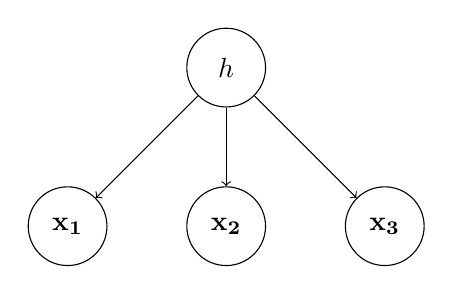
\begin{tikzpicture}[
  vertex/.style={draw,circle,minimum size=1cm},
  every node/.style={vertex}
  ]
	 \node (h) at (0,0) {$h$};
	  \node [below = of h] (x2) {$\vek{x_2}$};
	 \node [left = of x2]  (x1) {$\vek{x_1}$};	
	 \node [right = of x2] (x3) {$\vek{x_3}$};
	 
	 \draw [->] (h) edge (x1) (h) edge (x2) (h) edge (x3);
\end{tikzpicture}
\caption{Graphical representation of conditional independence relation between random variables $\vek{x_1, x_2, x_3}$ and $h$.}
\label{fig:graph}
\end{figure}

\end{document}  